% This is lnicst.tex the demonstration file of the LaTeX macro package for
% Lecture Notes of the Institute for Computer Sciences, Social-Informatics 
% and Telecommunications Engineering series from Springer-Verlag.
% It serves as a template for authors as well.
% version 1.0 for LaTeX2e
%
\documentclass[lnicst,a4paper]{svmultln}
%
\usepackage[english]{babel}
\selectlanguage{english}
%
\usepackage{svg}
%
\usepackage{wrapfig}
%
\usepackage{amsmath}
%
\usepackage{gensymb}
%
\usepackage{graphicx}
\DeclareGraphicsExtensions{.pdf,.svg,.jpg,.png,.eps} % first try pdf, then eps, png and jpg
%
\usepackage{makeidx}  % allows for indexgeneration
% \makeindex          % be prepared for an author index
%
\setlength{\textheight}{645pt}

\begin{document}
%
\mainmatter              % start of the contribution
%
\title{Humanoid Robot Obstacle Recognition via Data Filtering, Localisation and Robot-to-Robot Communication in Context of RoboCup} 
%
\titlerunning{Humanoid robot obstacle recognition}  % abbreviated title (for running head)
%                                     also used for the TOC unless
%                                     \toctitle is used
%
\author{Daniel Speck, Benjamin Scholz, Judith Hartfill}
%
\authorrunning{Daniel Speck, Benjamin Scholz, Judith Hartfill}   % abbreviated author list (for running head)
%
%%%% list of authors for the TOC (use if author list has to be modified)
\tocauthor{}
%
\institute{University of Hamburg, Fachbereich Informatik\\
\email{2scholz@informatik.uni-hamburg.de, 2speck@informatik.uni-hamburg.de, 2hartfil@informatik.uni-hamburg.de}
}

\maketitle              % typeset the title of the contribution
% \index{Ekeland, Ivar} % entries for the author index
% \index{Temam, Roger}  % of the whole volume
% \index{Dean, Jeffrey}




%%%%%%%%%%%%%%%%
%%%          %%%
%%% Abstract %%%
%%%          %%%
%%%%%%%%%%%%%%%%

\begin{abstract}        % give a summary of your paper
In RoboCup Soccer an intelligent behaviour is needed to be successful. This can be achieved with communicating robots to make team play possible. For team play and path planning a shared world model is required as well as the information of objects \& obstacles inside this world model. To locate those entities accurate data has to be supplied and this makes filtering necessary.
\\
The location is done via a grid world and for filtering a customized DBSCAN algorithm is used as well as an artificial neural network.
\\
The communication uses the mitecom standard.

%                         please supply keywords within your abstract
\keywords {obstacle recognition, obstacle avoidance, localisation, filtering, clustering, data smoothing, vision, swarm intelligence, grid world, DBSCAN, artificial neural network, multilayer perceptron, robotics, mitecom}
\end{abstract}
%




%%%%%%%%%%%%%%%%%%%%
%%%              %%%
%%% Introduction %%%
%%%              %%%
%%%%%%%%%%%%%%%%%%%%

\section{Introduction}

In this project our aim was to implement obstacle recognition for a team of robots taking part in the RoboCup Soccer Humanoid Kid Size League. So far each robot in the team made decisions dependent on its own information only such as the field of vision. This led to a decision making being dependent on one robot's limited individual data.
\\
Our objective was to develop modules which share data between all team mates for realizing an intelligent behaviour via localisation and mapping obstacles in this world model.
\\
For implementing such modules it is required to have sufficient vision data of the environment. Gathering this information we noticed that the supplied quality does not match this task's demands.
\\
Furthermore the position data of the robot and other objects data was noisy, so data filtering was necessary.
\\
Intelligent behaviour requires a world model which provides its information in a transformable and unique way between modules or even robots. Fulfilment of this task requires an internal team communication system contributing one robot's information for every team member.
\\
Thus a form of swarm intelligence could increase the quality of the robots acting together as a whole team by increasing the quality of information.
\\
Playing football always requires communication, so sharing information improves the team's efficiency. Transferring this key aspect of football to the software was one of our main ambitions.


\subsection{Comments on group work \& split of labour}
In this project we had a good cooperation, team work and several team discussions. Thus the results can not completely be split and allocated to a single person. We worked together as one team on most topics. Still we reflected our process and name the main persons for each part.
\\
Thus it appeared that the subjects "Vision" and "Filtering" primarily were done by Daniel Speck. He had the ideas and developed the approaches of our fixed vision and our filtering via DBSCAN and neural networks. Then the team discussed the plans and together with Benjamin Scholz and Judith Hartfill, Daniel Speck created a concept. The implementation on those topics was done by Daniel Speck.
\\
Looking at the "Localisation" and "Communication" chapter, such a strict seperation is not possible anymore. Most of these two topics were done by Benjamin Scholz and Judith Hartfill together.
\\
The idea to create a Gridworld came from Daniel Speck at another team discussion, but the concept and the implementation was done by Benjamin Scholz and Judith Hartfill.
\\
The idea for the communication part came from Judith Hartfill. The concept and implementation of it was done by Judith Hartfill and Benjamin Scholz.
\\
The testing and debugging for each of the topics was done jointly by all of us.
\\
In our paper the abstract, the first introduction part, the motivation and the summary were written as a team.
\\
The subsections ~\ref{sec:problems_vision}, ~\ref{sec:solutions_vision}, ~\ref{sec:results_vision} "Vision" and ~\ref{sec:problems_filtering}, ~\ref{sec:solutions_filtering}, ~\ref{sec:results_filtering} "Filtering" under the sections "Problems", "Solutions" and "Results" were written by Daniel Speck.
\\
The subsections ~\ref{sec:problems_localisation}, ~\ref{sec:solutions_localisation}, ~\ref{sec:results_localisation} "Localisation" under the sections "Problems", "Solutions" and "Results" were written by Benjamin Scholz.
\\
The subsections ~\ref{sec:problems_communication}, ~\ref{sec:solutions_communication}, ~\ref{sec:results_communication} "Communication" under the topics "Problems", "Solutions" and "Results" were written by Judith Hartfill.




%%%%%%%%%%%%%%%%%%
%%%            %%%
%%% Motivation %%%
%%%            %%%
%%%%%%%%%%%%%%%%%%

\subsection{Motivation}

Obstacle recognition and dynamic behaviour, specifically pathfinding towards or around obstacles is important if several robots shall act together as a team in a certain way to achieve specified goals.
\\
Team play/efficiency, fair play and hardware costs are the main reasons for intelligent obstacle recognition. One aspect of fair play is to avoid the physical contact between robots and as long as their hardware sometimes loses balance when the robot is touched, it is very likely to fall and - in worst-case-scenario - causes other robots downfall. Such collisions usually cause high costs for hardware fixes and also disturbs the gameplay. Getting up again takes several seconds and in addition it is not within the meaning of fairplay. Furthermore physical contacts are not compliant to the rules.
\\
Moreover and especially better knowledge about the surroundings is strategically important in the RoboCup competition. Having a reliable prospect of its own position, the position of the ball and the opponents' position combined with adequate path finding algorithm can raise the number of scores significantly.
\\
Those aspects cause a big increase in making the robot football play more realistic and authentic, which is the main aim of the RoboCup competitions.




%%%%%%%%%%%%%%%%
%%%          %%%
%%% Problems %%%
%%%          %%%
%%%%%%%%%%%%%%%%

\section{Problems}

\subsection{Vision}
\label{sec:problems_vision}
For an intelligent obstacle recognition several sufficiently pre-processed data input is needed to localise the obstacle itself, localise the robot itself, classify the obstacle (ball, goal, team-mate, enemy, other obstacle) and develop an adequate strategy of (re-)action.
\\
One of our first problems was the already implemented algorithm for obstacle and goal detection. We discovered that neither obstacles nor goals were tracked/recognized satisfactorily for our tasks.
\\
The obstacle detection was too imprecise to fulfil our plans of an intelligent reaction and the biggest problem was the missing localisation of the robot itself which is realized by tracking the goals (via tracking the two goal posts). Even when the robot stands completely still in a distance of two metres directly in front of the goal the vision detects four to six goal posts most of the time.
\\
The majority of false positives were shadows of the real posts or random mirages/reflections on the walls. This resulted in "jumping" goal posts because for the behaviour two posts are selected and out of the four to six possible posts the selection process to distinguish between the possibilities was not stable.
\\
In addition to that even when the real goal posts could be identified for several frames the algorithm often was not able to calculate the correct relative distances to the goal posts.
\\
The algorithm was designed to draw a rectangle over a possible goal post but it has no specific filters for the dimensions. This leads to rectangles having a wrong position, height and width compared to the original post. Some recorded datasets showed rectangles with twice or half the size of the real post and positional failures of several 10 centimetres.
\\
Appropriately reacting behaviour systems e.g. for intelligent obstacle recognition, localisation and further path planning or even post-processing filters would fail on such raw data.


\subsection{Filtering}
\label{sec:problems_filtering}
The whole topic of obstacle recognition relies on information which is extracted from (heavily) noisy input data.
\\
For our solutions primarily the goal post data and the later calculated goal centre information is important to calculate real, absolute coordinates for localisation purposes on the field out of the relative camera input.
\\
The raw data of goal posts (relative tuples of $x, y$ coordinates) when recorded over several seconds (with a still standing robot) often showed a spread distribution of points in a circle with a radius of about a quarter of a metre. Those datasets of 100 to 200 recorded samples had a standard deviation of 200 millimetres and above.
\\
Having such noisy data renders absolute positioning tasks and intelligent obstacle recognition (avoidance in case of real obstacles, path planning in case of balls) impossible.
\\
Since the robots do not have auto-calibration features the calibration of the camera and motor angles deteriorate the noise problem. Once the calibration is manually done its configuration is static but the real values vary over time, for example when the robot falls by accident.
\\
In addition to that the manual calibration is expansive in terms of time.


\subsection{Localisation}
\label{sec:problems_localisation}
Detecting an obstacle isn't worth much without knowing our own robot's position on the field. Of course the robot could avoid the recognised obstacle, but there is no way of knowing if it benefits our team in this situation. If the robot bypasses an opponent but actually walks in the wrong direction we haven't gained anything. 
\\
Also there is no way of knowing what robots are our team members and which one are our opponents.
\\
If the robot had all this data it could make more intelligent decisions and improve the flow of play.
\\
To achieve these goals we need a world model we can store information in, like our own position and the position of our team members and opponents.


\subsection{Communication}
\label{sec:problems_communication}
When thinking about how to achieve most and best information for each robot, we thought about swarm intelligence mechanisms. Although the Darwin-OP platforms that we use do have a lot more computing capacity then usual swarm intelligence bots have, we still can benefit from researches in this part of robotics. 
\\
Particularly as communicating, which is the basis for any smart intelligence, is a very important part in "real" human soccer, extending this aspect makes robot soccer even more humanoid, although Wi-Fi is a very unnatural (nevertheless not unhumanoid) way to communicate. In the future communicating vis Wi-Fi is going to be substituted by communicating via natural speech and speech comprehension, but getting started with this slightly simpler form is very important for the development.
\\
Until then, the robots only shared their own relative position to ball with each other. This was used to offset the lack of real localisation, especially the problem of symmetry. When a striker went towards the own goal with a ball, thinking it was te opponent goal, his own goalie would also see the ball and in return send its relative position to the ball. In case the distance between goalie and ball was less then half the field length, the striker could be quite sure to be playing onto its own goal and turned around. 
\\
But to use the whole capability of communication, shared information and thus interaction, we need a way to decode and encode information and to integrate received data with own data.




%%%%%%%%%%%%%%%%%
%%%           %%%
%%% Solutions %%%
%%%           %%%
%%%%%%%%%%%%%%%%%

\section{Solutions}





%%%%%%%%%%%%%%
%%%        %%%
%%% Vision %%%
%%%        %%%
%%%%%%%%%%%%%%

\subsection{Vision}
\label{sec:solutions_vision}
The vision's detection of obstacles and objects is based on a horizon scanning algorithm which tries to find the horizon in the current frame. Basically it reads the pixel information of the current frame in matrix and finds the specific row where the horizon is located.
Once this row is found the algorithm for obstacle detection scans down to find "green" pixels for locating the field. Every obstacle, for example the goal posts, create non-green shapes in this matrix.


\subsubsection{Goal information}
The algorithm searches for the yellow colour mask of the goal posts to detect every goal post in the current frame. For every potential goal post which is found the algorithm tries to extrapolate the shape of the goal post and to fit a virtual rectangle with nearly the same dimensions on it.
\\
Often the width of the rectangle was calculated wrong (being twice or half as big as the original post). This failure exists because of image distortions which manipulate the object's shapes and the angle at which the object is seen (basically the bottom of the object is wider, the top thinner because of the angle).
\\
This problem basically remains but with modified parameters we were able to make the fitting of the virtual rectangle more strict. Those changes slightly improved the rectangle width compared to the real goal post.
\\
In addition to that the implemented algorithm now searches the bottom of the object by scanning down to one of the objects last lines in the matrix. This solution relatively stabilizes the problem because the previous algorithm just picked some line of the top of the object compared to the horizon line in the current frame and those information varies much more (top \& horizon line) in dependency of the camera angle compared to the objects bottom (green and non-green contrast on the field).
\\
Scanning for the bottom of the object is even more profitable when it comes to the height of the object because the bottom of a goal post (yellow) and the field (green or white) always have a hight contrast change so the bottom line is found reliably.
\\
To further improve the detection of the goal posts we finally modified the algorithm not to take a corner of the virtual rectangle but to calculate the centre of the bottom line. This approach is more stable because the error is halved when the width of the virtual rectangle changes.


\subsubsection{Obstacle information}
The obstacle detection also scans downwards starting at the horizon line in the current frames matrix. Abnormal contrast changes are interpreted as obstacles if its size is large enough.
\\
Objects like the ball are filtered by another algorithm. A point cloud filtering and an orange colour map are detecting the ball.
\\
Arbitrary coloured obstacles with a significant size are classified as miscellaneous obstacles. Those obstacles are "real" obstacles which should be avoided (in case of a human on the field or an enemy robot) or blocked (in case of an enemy with the ball trying to score at our goal).
\\
This obstacle information is processed separately and can be filtered to stabilize its data / position. This data is later mapped into our grid world model.




%%%%%%%%%%%%%%%%%
%%%           %%%
%%% Filtering %%%
%%%           %%%
%%%%%%%%%%%%%%%%%

\subsection{Filtering}
\label{sec:solutions_filtering}

\subsubsection{Data noise}

%\begin{wrapfigure}{r}{0.6\textwidth}
%  \begin{center}
%    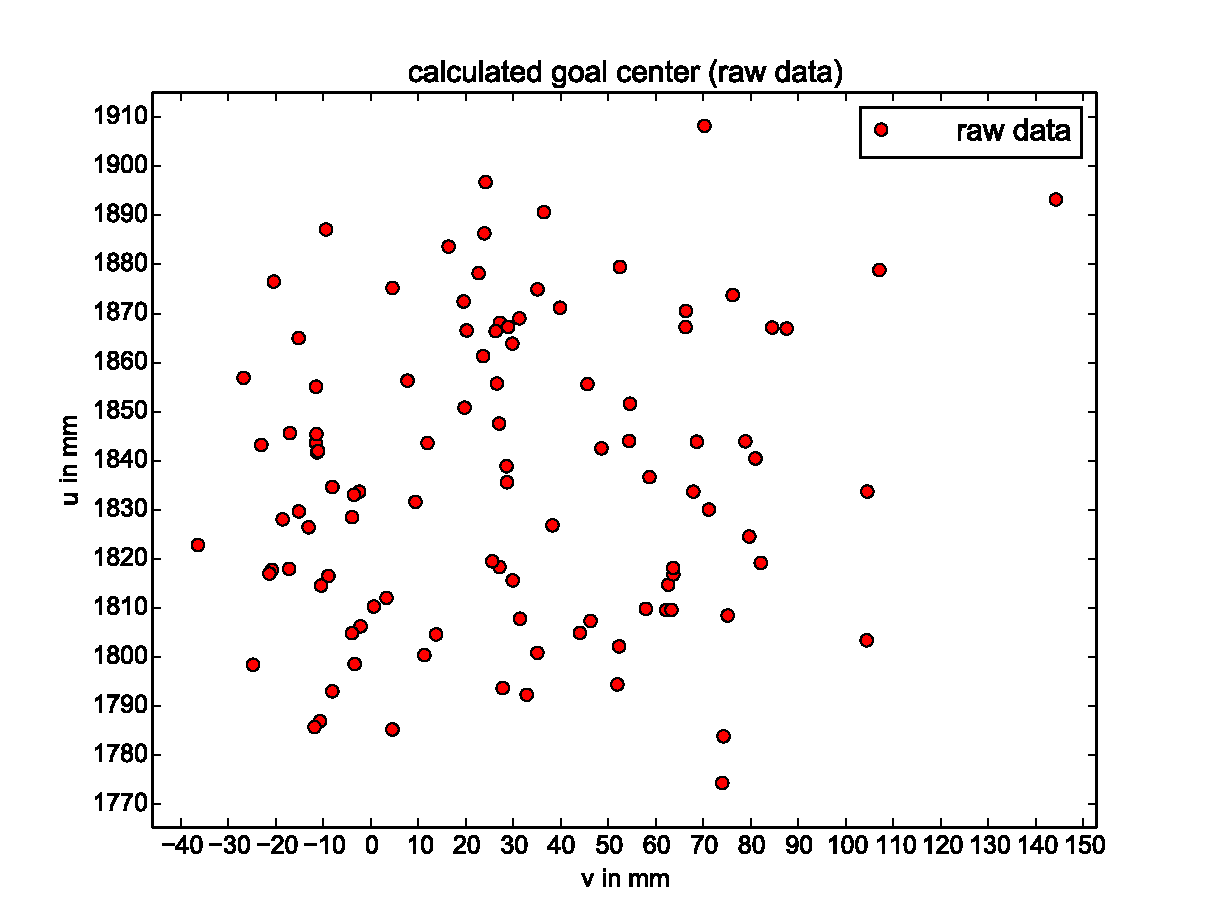
\includegraphics[width=0.58\textwidth]{noise_data_plot.pdf}
%  \end{center}
%  {\caption{Plot of raw goal center data (100 data sets recorded in about 5 seconds) without filtering and calibration. Original vertical distance to goal center was 2000mm and horizontal distance 0mm. The robot was standing still.}
%  \label{fig:noise1}}
%\end{wrapfigure}

The majority of the bitbots code works without filters on raw data, especially in the case of goal information no post-processing exists.
\\
The goal information (goal post positions and goal centre position) is needed to localise the robot on the field in our case. Intelligent behaviour according to obstacle recognition relies on this localisation (our grid world module) so the goal information is the most important data for our software and has to be as accurate as possible.



\begin{figure}
 	\centerline{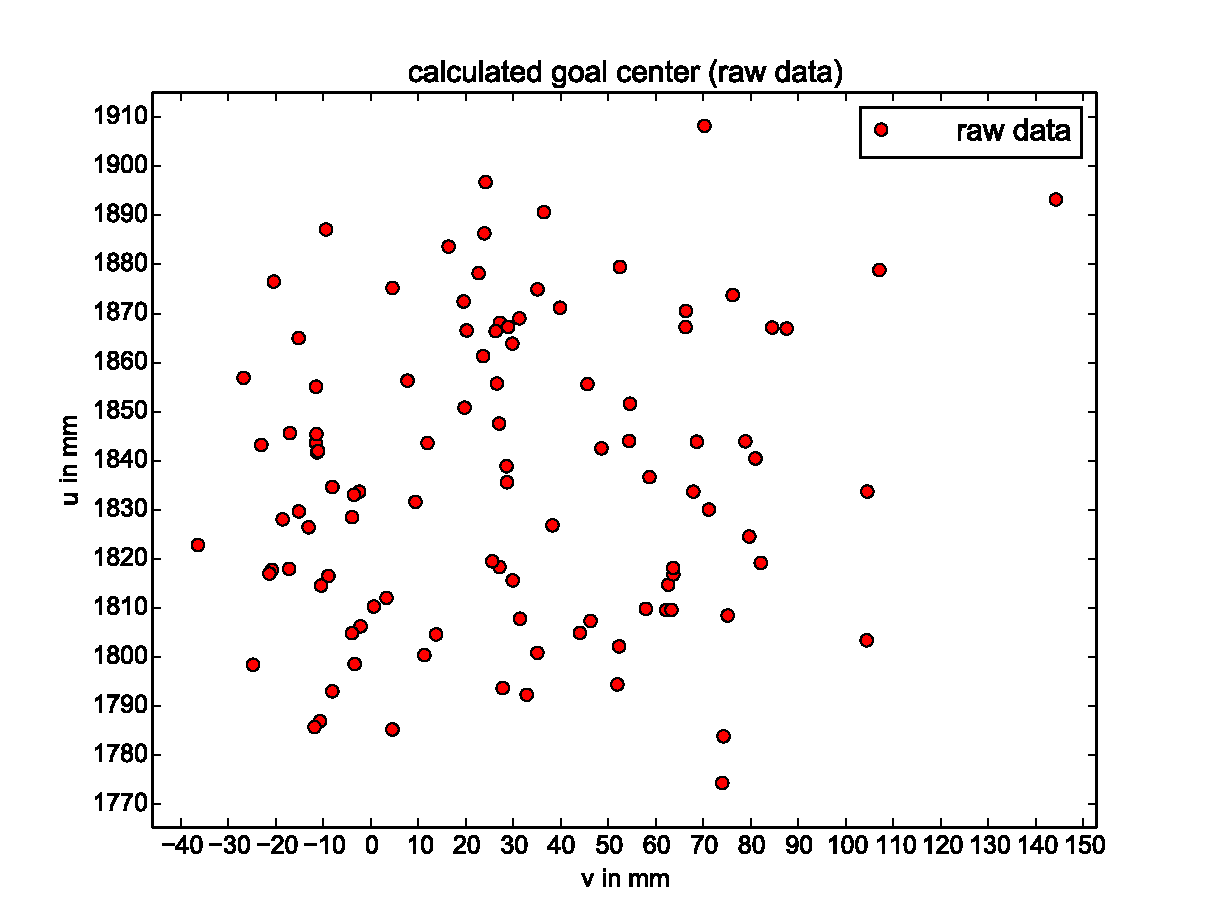
\includegraphics[width=0.7\textwidth]{noise_data_plot.pdf}}
	{\caption{Plot of raw goal centre data (100 data sets recorded in about 5 seconds) without filtering and calibration. Original vector to goal centre was $(2000$  $0)^T$. The robot was standing still. The goal center (purple) and robot (black) were placed in the plot afterwards.}
	\label{fig:noise1}}
\end{figure}

As shown by figure~\ref{fig:noise1} the noise of the raw data in combination with missing calibration is too high to allow an accurate localisation.
\\
We define a distance vector $\vec{d} := \left( \begin{array}{cc} u & v \end{array} \right)^{T}$ to contain the horizontal ($u$) and vertical ($v$) distance to a point relatively to the robot's position. 
\\
The vector 
$\vec{d_{0}} := \left( \begin{array}{cc} 2000 & 0 \end{array} \right)^{T}$ is the real vector to the goal centre and vectors like
$\vec{d_{1}} := \left( \begin{array}{cc} 1797 & -25 \end{array} \right)^{T}$ and
$\vec{d_{2}} := \left( \begin{array}{cc} 1877 & 107 \end{array} \right)^{T}$
are the vectors of two recorded points shown in figure~\ref{fig:noise1}.
\\
The euclidean distance $ed$ between two vectors $\vec{a}, \vec{b}$ is calculated by equation~\ref{equ:euclidean_distance}:
\\
\begin{equation}
\label{equ:euclidean_distance}
ed = \sqrt{\sum_{i=1}^{n} (a_i - b_i)^2}
\end{equation}
\\
For two dimensional problems $n$ of equation~\ref{equ:euclidean_distance} is 2. Herewith we can calculate the differences between the vectors.
\\
$\vec{d}_{0}$ differs to $\vec{d}_{1}$ by
$ 204 = \sqrt{(2000 - 1797)^2 + (0 - (-25))^2}$ and 
$\vec{d}_{0}$ to $\vec{d}_{2}$
by $ 163 = \sqrt{(2000 - 1877)^2 + (0 - 107)^2}$
in euclidean distance.
\\
Those differences are too large to ensure a correct mapping in our grid world module as the differences occurred in less than three seconds while the robot was standing still. In addition the vertical difference between $\vec{d}_{1}$ and $\vec{d}_{2}$ is $ 134 = |-27| + 107 = |-27| + |107|$. Recordings of several seconds show the mentioned noise distribution in a circle of about a quarter of a metre.
\\
Nevertheless clusters of points can be detected in figure~\ref{fig:noise1} and this is the reason why we decided to filter the data via a DBSCAN algorithm.


\subsubsection{DBSCAN}
Our approach to reduce the noise on data was implementing a two dimensional version of the DBSCAN (density-based scanning) algorithm \cite{ester:kriegel}, which we slightly customized to our needs.
\\
At first our code was an exact re-implementation in pure Python of the DBSCAN algorithm \cite{ester:kriegel}
originally proposed by Martin Ester et al. in 1996 but this procedure was just for testing to assure the algorithm meets our requirements.
\\
Due to the performance issues of pure Python implementations we refactored the complete code and made use of Numpy (mainly) and other SciPy libraries. As a consequence of the C/C++ core implementations of those libraries the overall execution time of our code decreased.
\\
In addition to that the refactored, performant version of our DBSCAN is implemented object oriented. This leads to an overhead in space complexity but offered easier debugging as well as an additional improvement of execution time because the calculations are saved in objects and those cached results are re-used as much as possible.
\\
In our tested cases the pure Python implementation ran about 8 to 12 times slower on average (dependent on current background tasks) on the darwin-op hardware compared to our current object oriented Python implementation with Numpy and other SciPy libraries.
\\
Those optimizations are essential considering the very limited computing power of the current darwin-op robots.
\\
For calculating the goal information each goal posts raw input data (if post is seen) is recorded separately in buffers of a maximum size of 60 items. Every new frame delivers one new data set and on average the robots architecture is able to handle about 20 frames per second. If a buffer is full, the oldest entry is dropped and the newest saved. As data structure for the buffers we chose Python Deque objects for easy appending and extracting data sets.
\\
If the robot changes its position, old data sets would mess up the calculation, so our DBSCAN object automatically drops data sets which are older than 10 seconds to prevent those kind of failures. Minor positional changes in the meantime are no problems in most cases, because the DBSCAN would filter those datasets appropriately.
\\
In figure~\ref{fig:dbscan_illustration1} a graphical illustration of the DBSCAN algorithm is shown.

\begin{figure}
 	\centerline{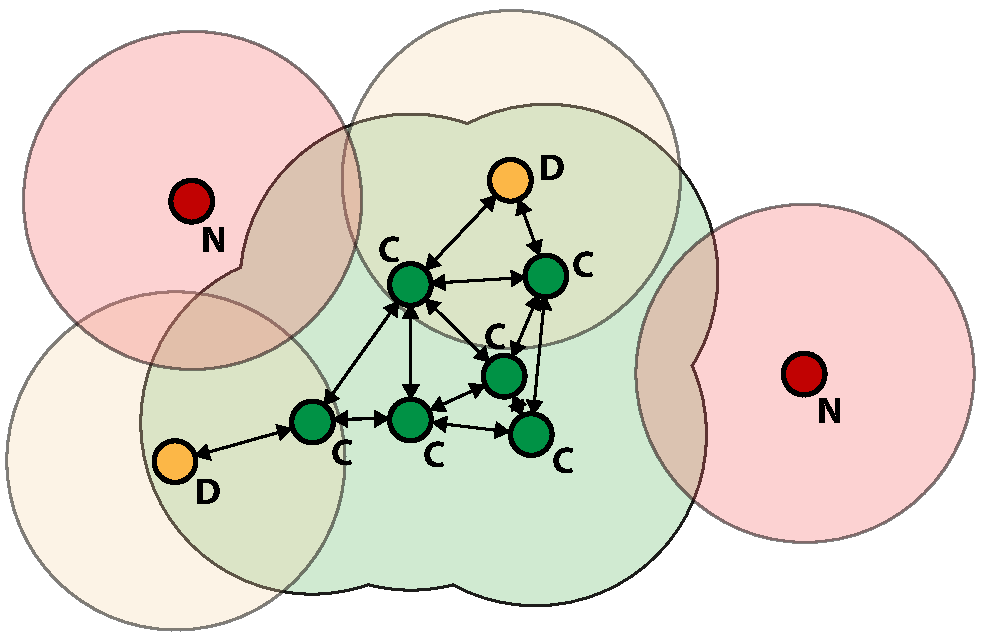
\includegraphics[width=0.7\textwidth]{dbscan1.pdf}}
	{\caption{DBSCAN graphical illustration.
	The points labelled with `C' are core points,
	the yellow ones labelled with `D' are density-reachable points
	and the red ones labelled with `N' noise points.
	The minimum points parameter is set to $4$ in this example.}\label{fig:dbscan_illustration1}}
\end{figure}

The DBSCAN algorithm has two parameters: the minimum points $\kappa$ (in some papers referred only with "minimum points"), which are required to initialize a new cluster and the radius $\epsilon$ in which neighbouring points should be searched.
\\
The point counts itself to its neighbourhood, too. Therefore every point has a $\kappa$ of at least 1.
\\
All points are two-dimensional and consist of the relative horizontal distance ($u$) and the relative vertical distance ($v$) to the object.
\\
At first DBSCAN marks every point as "unvisited". In the next step the algorithm chooses one point $p_0$ at random, marks it as "visited" and searches in his neighbourhood for neighbouring points within its $\epsilon$ radius. This is done by calculating the euclidean distance (see equation~\ref{equ:euclidean_distance}) between the points.
\\
This procedure would find all points within a circle with the radius of $\epsilon$ as shown in figure~\ref{fig:dbscan_illustration1}. If the amount of found neighbouring points in neighbourhood to $p_0$ is greater or equal to $\kappa$, than a new cluster is initialized. Otherwise the point is would be marked as "noise".
\\
A newly initialized cluster would then continue with the next point $p_1$ within the cluster and also mark it as visited as well as search for other neighbouring points in $p_1$'s $\epsilon$ neighbourhood. This continuation stops when all points in the cluster are processed, so the cluster is expanded to its maximum size like the green cluster in figure~\ref{fig:dbscan_illustration1}.
\\
Points within the cluster's range which do not fulfil the precondition of its neighbourhood being greater or equal than $\kappa$ are marked as "density-reachable" points. Those points are not part of the original cluster but in range so the point is considered to be better than pure noise because of a cluster being in its $\epsilon$ radius.
\\
This process loops through all data sets, finds the clusters and continues until every point is marked as "visited" and classified as either "core", "density-reachable" or "noise".

\begin{figure}
 	\centerline{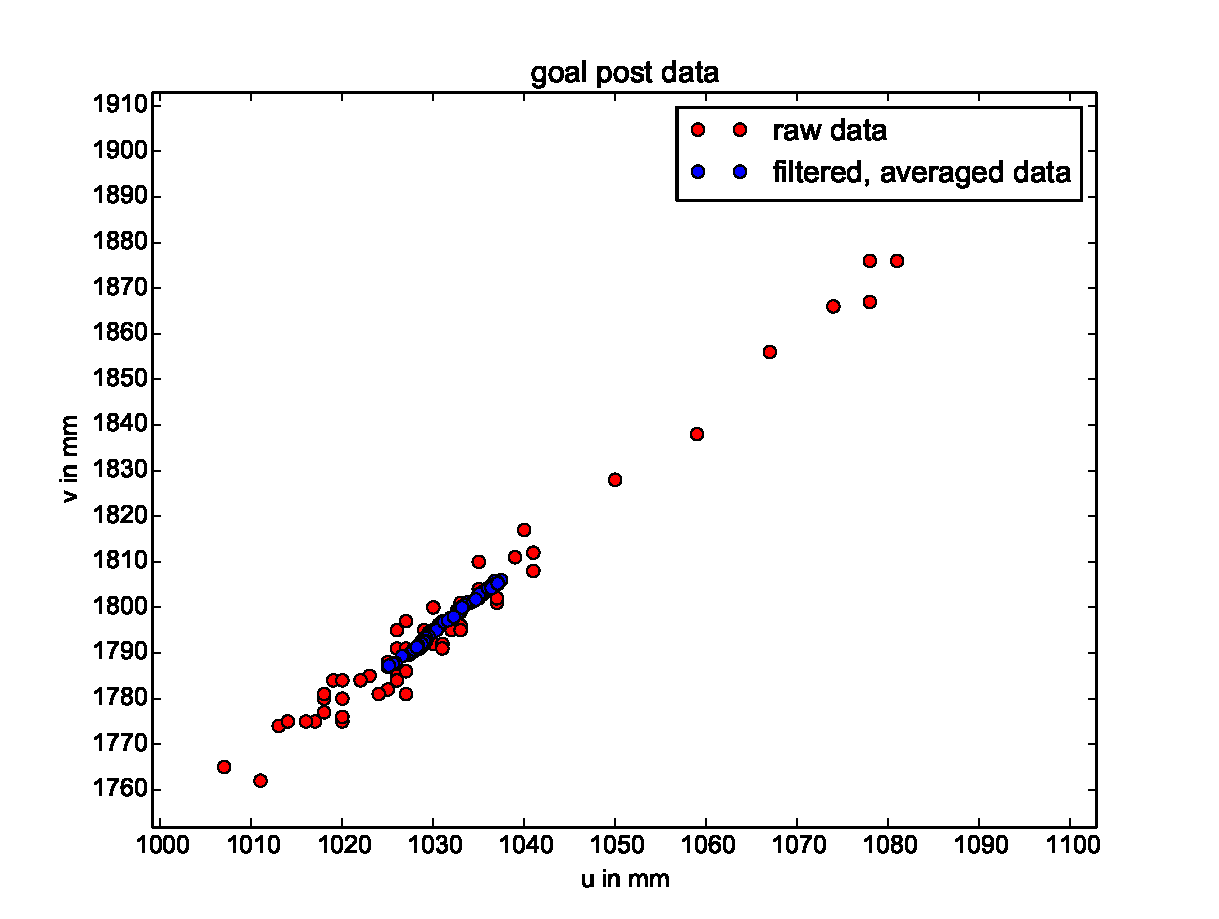
\includegraphics[width=0.7\textwidth]{dbscan_data_plot1.pdf}}
	{\caption{Plot of DBSCAN-filtered and averaged data. Recorded object was a goal post to the right of the robot. 100 data sets have been recorded in about 5 seconds. Original vertical distance (v) to the post was 1000mm and horizontal distance (u) 2000mm. The robot was standing still.}\label{fig:dbscan_plot1}}
\end{figure}

Throughout our testing process we experienced positive results with a $\kappa$ of 6 and an $\epsilon$ of 50 as parameters for our DBSCAN implementation.
\\
After our DBSCAN has processed all data it returns the found clusters and density-reachable points. Those data is not directly returned to modules requesting filtered data.
Before sending the filtered data our filter module calculates the arithmetical mean for every cluster plus density-reachable points.
\\
Figure~\ref{fig:dbscan_plot1} shows a dataset of 100 red unfiltered points and the filtered and averaged blue points. The euclidean distance between the filtered points is decreased heavily and outliers are reliably marked as noise and therefore not processed nor averaged.
\\
Nevertheless the goal post information may be sufficient for some purposes, but at least for the goal centre calculation this is not sufficient. Due to calibration issues and the distribution of noise the goal centre calculation would not be optimal then calculated out of this data directly.
\\
For this purpose, to further improve the stability and precision of goal centre information, we implemented an artificial neural network.

\subsubsection{Artificial Neural Network}
For fixing the calibration issues and more accurate data our idea was to implement an artificial neural network (multilayer perceptron design).
\\
\begin{figure}
 	\centerline{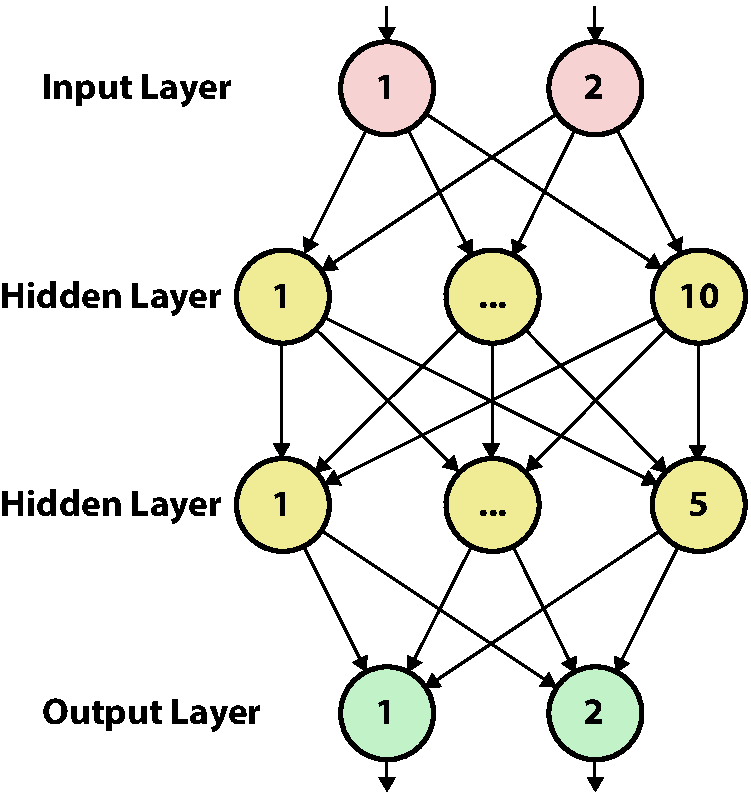
\includegraphics[width=0.7\textwidth]{neuralnet1.pdf}}
	{\caption{Illustration of our Artificial Neural Network design (multilayer perceptron).}\label{fig:ann_illustration1}}
\end{figure}
\\
The module is designed object oriented and caches every calculation to prevent something being calculated twice. This, again, increases the space complexity but decreases the computing time and was simpler in cases of debugging, too.
\\
In addition to this the whole data (weights, bias, activations, outputs, ...) is stored in Numpy arrays and always calculated with Numpy matrix operations or scalars to save as much computation time as possible.
\\
Furthermore the neural network is designed dynamically. All configurations are alterable. At the moment our network has an input layer with 2 neurons, 2 hidden layers with 10 and 5 neurons and an output layer with 2 output neurons. The learning rate $\epsilon$ is $0.2$ with $20,000$ learning steps and $1,000$ training data sets.
\\
All this configurations can be changed instantly, for example a Python list of integers $[10, 5]$ represents the hidden layers at the moment and can be changed to $[20, 10, 5]$ at any time, which would create a net with 3 hidden layers with 20, 10 and 5 neurons per layer.
\\
In addition to this our neural network class can save its configuration (trained weights and bias, layers and neurons) by encoding the arrays via base64 and dumping all Python and Numpy Array information with JSON. This encoded string has a length of about 20 lines and is written in a file. The class is able to read this file, decode the information and rebuild itself automatically.
\\
In figure~\ref{fig:ann_illustration1} our multilayer perceptron design is illustrated. Overall it follows the standard MLP design \cite{mlp}. Each layer is fully connected to the parents layer. As a transfer function we use hyperbolic tangent ($tanh$) as well as its derivation for learning which is realized via supervised learning with backpropagation.
\\
In contrast to the standard feedforward activation we implemented a customized version. The standard feedforward activation:
\\
\begin{equation}
\label{equ:mlp_feedforward_standard}
h_{i}^{\lambda} (\vec{w}_{i}^{\lambda \lambda-1})
=
\sum\limits_{j} w_{ij}^{\lambda \lambda-1} s_{j}^{\lambda-1} + b_{i}^{\lambda}
\end{equation}
\\
$h_{i}^{\lambda}$ is the whole activation of neuron $i$ in layer $\lambda$. The weights of neuron $i_{\lambda}$ are described by $\vec{w}_{i}^{\lambda \lambda-1}$, so this represents the weights between the current neuron of current layer $\lambda$ and the parents neuron of parent layer $\lambda-1$. The output of each neuron for layer $\lambda-1$ is $s_{j}^{\lambda-1}$, so the parent layers neurons are indexed with $j$. Finally the bias $b_{i}^{\lambda}$ is added to create a kind of threshold.
\\
The neuron output of a neuron $i_{\lambda}$ then simply is the activation corrected by the transfer function:
\\
\begin{equation}
\label{equ:mlp_neuron_output}
s_{i}^{\lambda} (h_{i}^{\lambda}) = tanh(h_{i}^{\lambda})
\end{equation}
\\
Testing equation~\ref{equ:mlp_feedforward_standard} for our neural network showed that the learning process takes a vast amount of time and steps.
\\
This happens because of the non-linear transfer function $tanh$ which is used to normalize the neuron's activation and our network design having 10 and 5 neurons in the hidden layers. The limes $\lim\limits_{x \to \infty} tanh(x)$ is 1 and because of the fully connected layers (see figure~\ref{fig:ann_illustration1}) and randomly initialized weights the activation $h_{i}^{\lambda}$ of one single neuron (which, as shown in equation~\ref{equ:mlp_feedforward_standard}, is the sum of the output of each parent layers neuron multiplied with the weights plus its bias) can be far higher than 1 so that the hyperbolic tangent function returns 1 for a long period of time for the output $s_{i}^{\lambda}$ of this neuron. This inhibits the learning / backpropagation.
\\
Considering this problem, the output of the hidden layers are near 1 for several hundreds, sometimes thousands of learning steps. This takes a vast amount of time until the weights would change to decrease the neurons output. Those learning steps will not improve the network but just deteriorate the results. 
\\
To fix this problem, we customized the activation function. Instead of simply adding all incoming activations from each parent layers neuron we took the average activation of the whole parent layer to ensure the activation will always be in the interval of $[-1.0, 1.0]$ (this interval produces far better results with $tanh$):
\\
\begin{equation}
\label{equ:mlp_feedforward_custom}
h_{i}^{\lambda} (\vec{w}_{i}^{\lambda \lambda-1})
=
\frac{
\sum\limits_{j} w_{ij}^{\lambda \lambda-1} s_{j}^{\lambda-1} + b_{i}^{\lambda}
}
{\eta^{\lambda-1}}
\end{equation}
\\
In our customized feedforward activation (equation~\ref{equ:mlp_feedforward_custom}), the $\eta^{\lambda-1}$ is the amount of neurons total in the parent layer $\lambda-1$. Dividing the activation by $\eta^{\lambda-1}$ ensures the whole activation of neuron $i$ to be in the interval of $[-1.0, 1.0]$ as mentioned.
\\
This method greatly reduced the needed learning time and steps of our network. The saved amount of time and steps increases with larger nets because the overall higher activation without this normalization would cause the hyperbolic tangent function to map the values nearly 1 for a longer time.




%%%%%%%%%%%%%%%%%%%%
%%%              %%%
%%% Localisation %%%
%%%              %%%
%%%%%%%%%%%%%%%%%%%%

\subsection{Localisation}
\label{sec:solutions_localisation}

\subsubsection{Calculating our robot's position}
The robot provides a lot of different data.
But unfortunately most of the values are not fixed points on the field and so they are unsuitable to calculate the robot's position. From the data given by the robot only the distances to the goal posts are sufficient for our purposes.
\\
But the information the robot actually provides is not the direct distance but only the distance in front of the robot and the distance to the left of the robot to the objects. We will call the distance in front of the robot u and to the left of it v to stay consistent with the terms used in the code. figure~\ref{fig:uvvalues} contains an example of these values.
\begin{figure}
 	\centerline{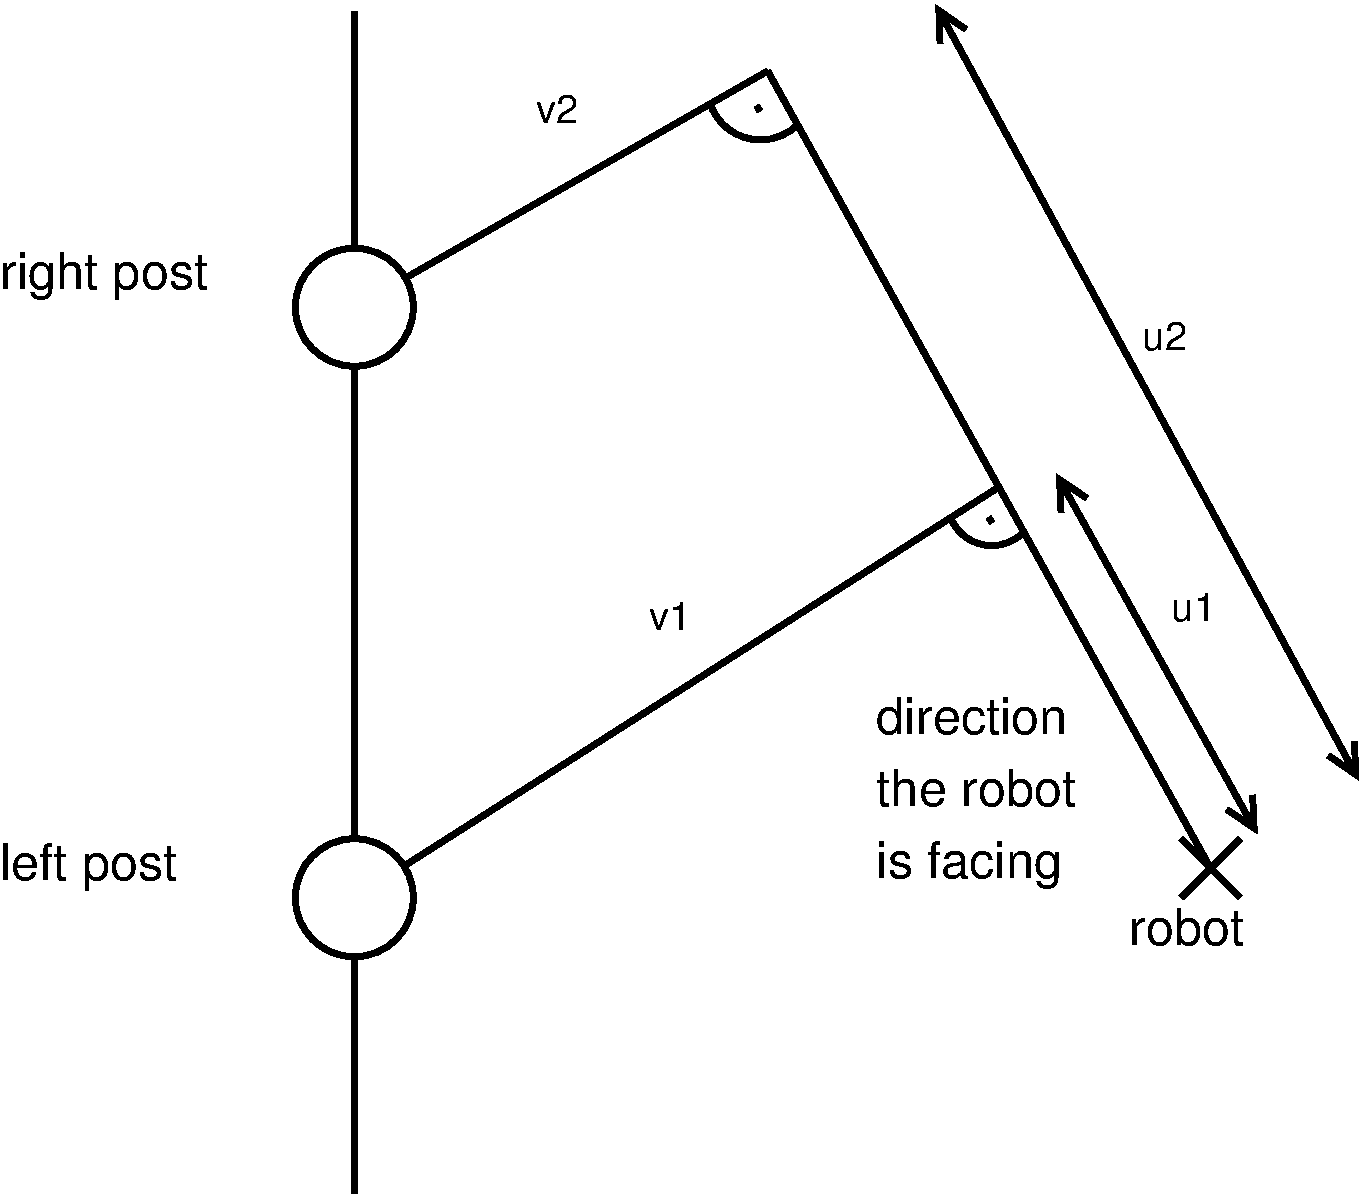
\includegraphics[width=0.7\textwidth]{uvvalues.pdf}}
	{\caption{Example of u- and v-values.}\label{fig:uvvalues}}
\end{figure}
\\
At first we want to outline how we basically calculated the position of our own robots and afterwards we are going to explain all steps in detail.
\\
For this calculation we used the u- and v-values to two goal posts. We use these values to calculate the direct distances to the goal and get two lines that intersect exactly at the robot's location. For this reason it's necessary to calculate the slope of the two lines so that we can form equations for them. With these we can determine the point of intersection. And once we know the point of intersection we also know the robot's position.
\\
For these calculations we need a coordinate system. That system is similar to the grid world, that we explain in a later segment. Meaning the origin is also at the mid point of the field and the opponent's goal is in the positive range on the x-axis and our goal is in the negative range. All following calculations are done in millimetre and later converted to the units of the grid world. Also we are going to assume that the robot faces the opponent's goal. 
\\
We are going to call the u- and v-values for the left post \(u_{1}\) and \(v_{1}\), and for the right post \(u_{2}\) and \(v_{2}\). You can use Pythagora's theorem to calculate the direct distances to the goal posts as done in equation~\ref{equ:distance}.
\begin{equation}
	d = \sqrt{u^2+v^2}
	\label{equ:distance}
\end{equation}
We do that for both goal posts and we are going to call the distance to the left post \(d_{1}\) and to the right post \(d_{2}\). 
\\
We want to know the angle between these lines and the goal width \(\psi\). The goal width doesn't change and we can retrieve it in the code, but the robot's goal post recognition can be very inaccurate. So even though in reality the goal width is always the same, according to the robot's values the goal width is changing all the time. So the robot calculates it's own value for the goal width too. We use the u- and v-values to create vectors and calculate a vector between the two goal posts:
\begin{equation}
	\vec{gw}=\left(\begin{array}{c} u_{1} \\ v_{1} \end{array}\right) - \left(\begin{array}{c} u_{2} \\ v_{2} \end{array}\right)
\end{equation}
The absolute value of the vector \(gw\) is the goal width \(\psi\).
\\
Now that we computed these three values we can form a triangle like in figure~\ref{fig:triangle}.
\begin{figure}
 	\centerline{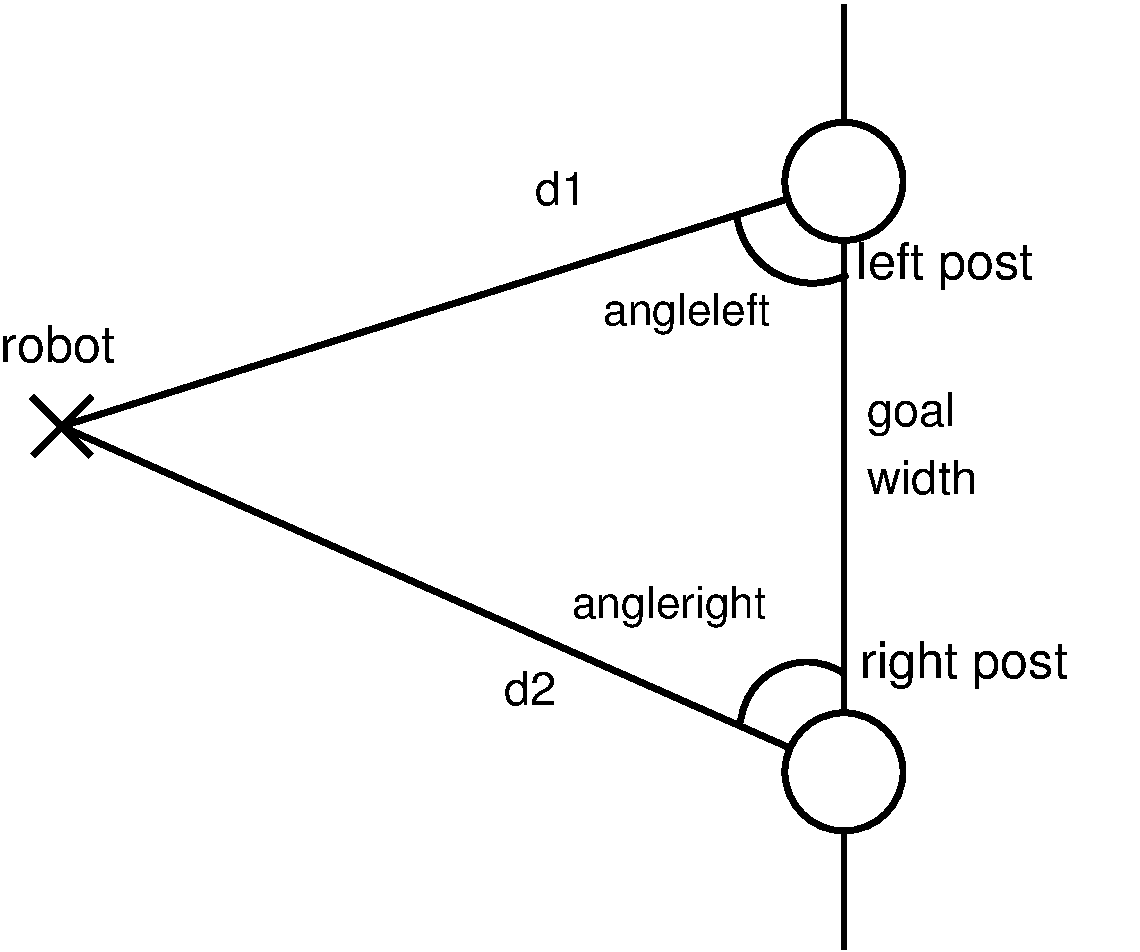
\includegraphics[width=0.6\textwidth]{triangle.pdf}}
	{\caption{}\label{fig:triangle}}
\end{figure}
\\
With the help of that triangle we are going to calculate the point of intersection of \(d_{1}\) and \(d_{2}\). 
\\ 
To calculate the point of intersection we need to form two equations for \(d_{1}\) and \(d_{2}\). In order to do that it's necessary to know the slope of both lines. 
\\
We calculate the two angles shown in figure~\ref{fig:triangle}.
The formula we used is the following:
\begin{equation}
	\alpha = \arccos{(\frac{a^2-b^2-c^2}{-2bc})}
	\label{equ:angle1}
\end{equation}
\\
Specifically these are the two formulas if you want to calculate the angle of the left post and the right post in the triangle:
\\
\begin{equation}
	angleleft = \arccos{\frac{(d_{2}^2 - d_{1}^2 - \psi^2)}{(-2*d_{1}*\psi)}}
	\label{equ:angleleft}
\end{equation}

\begin{equation}\
	angleright = \arccos{\frac{(d_{1}^2 - d_{2}^2 - \psi^2)}{(-2*d_{2}*\psi)}}
	\label{equ:angleright}
\end{equation}
\\
To convert the angles to the slopes of the two lines in the coordinate system, we can do the following:\\
\begin{equation}
	sloperight = (-1)*\frac{1}{\tan{angleright}}
	\label{equ:sloperight}
\end{equation}
\\
On the left side we don't need the angle itself but the angle above the line, which is 180\(\degree\) - angleleft:
\begin{equation}
	slopeleft = (-1)*\frac{1}{\tan{(180\degree - angleleft)}}
	\label{equ:slopeleft}
\end{equation}
Because we want to know the point of intersection of these two lines we need equations for them:
\begin{equation}
	y_{1} = slopeleft * x + b_{1}
	\label{equ:y1}
\end{equation}
\begin{equation}
	y_{2} = sloperight * x + b_{2}
	\label{equ:y2}
\end{equation}
\(b_{1}\) and \(b_{2}\) are the points of intersection with the y-axis. Our coordinate system has it's point of origin at the middle point of the field. As stated the reason for that is that the origin of our grid world is at that point as well, so it's easier to convert the values later on.
\\
We know the x- and y-values at the points of the goal posts. It is half the field length for both x-values and half the goal width for \(y_{1}\) and minus half the goal width for \(y_{2}\). With these points we can determine the values for \(b_{1}\) and \(b_{2}\) by rearranging the formulas. Afterwards we equate the equations ~\ref{equ:y1} and ~\ref{equ:y2} and solve this new equation for x. Then we can enter the found x-value in one of the two formulas to determine y. The found x- and y-value is the position of the robot in the coordinate system.
\\
\subsubsection{Calculating our robot's angle to the x-axis}
Now the robot knows its own position. But it can't determine the opponent's position on the field yet, because it doesn't know which direction it faces. The robot has its own inner coordinate-system. (0,0) is the middle of the robot. The orientation of the y-, and x-axis depend on the direction the robot faces.\\
So at first we calculate how many degrees the robot would have to turn to face one of the two goal posts. If the robot turns to that angle and would walk directly to the goal post he would end up directly in front of it, but not looking directly at it. To achieve that we need another angle. Now if the robot would turn that angle he would look directly at the goal post. So all we need to do at the end is, according to the exact situation at hand, either add or subtract the two angles we calculated and we would know the angle to the x-axis.
In figure~\ref{fig:angles} the first angle we mentioned is \(\beta_{2}\) and the second one is new\_angle\_right.
\begin{figure}
 	\centerline{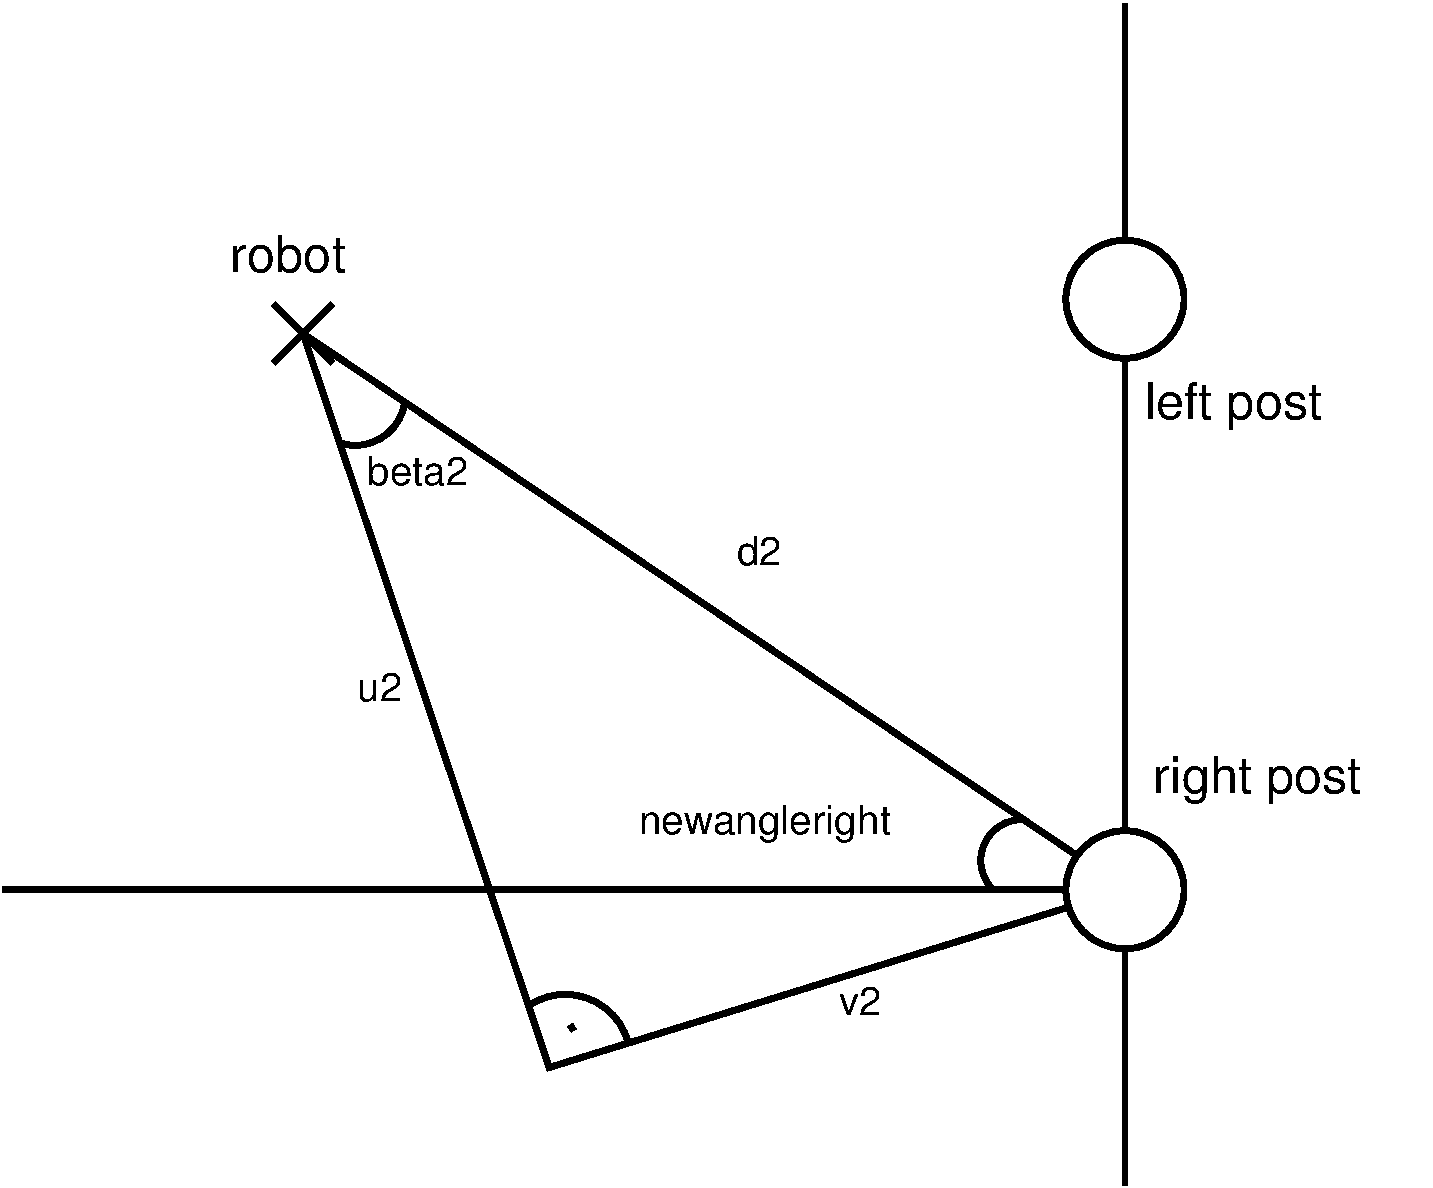
\includegraphics[width=0.6\textwidth]{angles.pdf}}
	{\caption{Example of angles needed to calculate the angle to the x-axis of our grid}\label{fig:angles}}
\end{figure}
\(\beta_{1}\) and \(\beta_{2}\) are calculated with the following equation:
\begin{equation}
	\beta = \arcsin{(\frac{v}{d})}
\end{equation}
We explained earlier how we calculated angle\_right and angle\_left. new\_angle\_left and new\_angle\_right are just 90\degree minus the old angles. 
\\
This only works if the old angle is under 90 degree, but this is always true for at least one of the two angles.
\\
Now there are different cases which affect how exactly we calculate the angle to the grid. At first we check if \(u_{1}\) or \(u_{2}\) is bigger. In our example we face the opponents goal. If \(u_{1}\) is bigger that means that the robot faces to the left and that the angle is smaller than 180\degree. In that case we just add \(\beta_{1}\) to new\_angle\_left.
\\
In the other case \(u_{2}\) is bigger and the robot faces to the right. In that case the angle to the x-axis has to be over 180\degree. We simply subtract \(\beta_{2}\) plus new\_angle\_right from 360\degree.
\\
So now that we know the position of the robots and their orientation we can finally calculate the position of other robots on the field.

\subsubsection{Calculating other robot's positions}
When our robot sees another robot it gets its distance as u- and v-values. Once again we can calculate the direct distance by using equation~\ref{equ:distance}. We want to use polar coordinates to calculate the position of the other robots. These consist of the direct distance \(r\) to the object and the polar angle \(\phi\), which is the angle between r and the x-axis of the grid in our case. 
\begin{figure}
 	\centerline{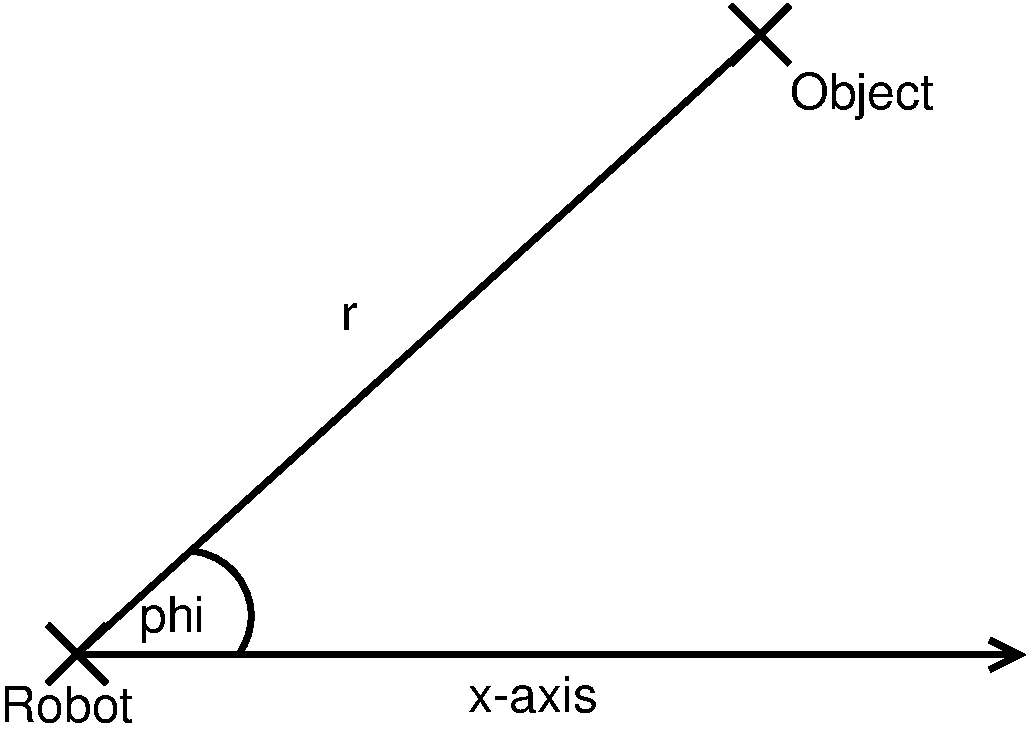
\includegraphics[width=0.6\textwidth]{polar.pdf}}
	{\caption{Example of r and \(\phi\)}\label{fig:polar}}
\end{figure}
In order to calculate \(\phi\) we need to know the angle from u to r. We use equation~\ref{equ:angle1} for this purpose, and substitute u for a, v for b and r for c. 
\\
We already determined the angle from the direction the robot is facing to the grid.
\\
To finally get the angle from the object to the grid we have to either add or subtract these two angles depending if the robot is left or right of the object, meaning if the v-value is positive or negative. So depending on the circumstances we use either equation~\ref{equ:a1} or equation~\ref{equ:a2}.
\begin{equation}
	\phi = (angle\_robot\_to\_grid - angle\_robot\_to\_object) \% 360
	\label{equ:a1}
\end{equation}
\begin{equation}
	\phi = (angle\_robot\_to\_grid + angle\_robot\_to\_object) \% 360
	\label{equ:a2}
\end{equation}
Afterwards we use equation~\ref{equ:x} and~\ref{equ:y} to determine the x- and y-values.
\begin{equation}
	x = r*\cos(\phi)
	\label{equ:x}
\end{equation}
\begin{equation}
	y = r*\sin(\phi)
	\label{equ:y}
\end{equation}
These values still depend on the position on the robot, so at the end we have to add the position of the robot to the found values to finally get the position of the other robot on the field.

%%%%%%%%%%%%%%%%%%
%%%            %%%
%%% Grid World %%%
%%%            %%%
%%%%%%%%%%%%%%%%%%

\subsubsection{Grid World}
Now that we know the positions of our own and other robots we need some way to save and share these positions, so that our team members can make use of that knowledge and every robot in our team can profit. We needed a representation of the field, so we could store and use the data we generated. For that purpose we use the grid world. Other approaches we considered were a coordinate system that uses millimetres and a tree based solution \cite{tree}. In the end we decided to use said grid world because of its simplicity and several advantages. Even though Daniel had the idea for that representation of the field it turns out we are not the first robocup-team to use it. \cite{grid} So we need to divide the field into a certain number of cells. As shown in figure~\ref{fig:gridworld} the origin of the cells is at the midpoint of the field.
\begin{figure}
 	\centerline{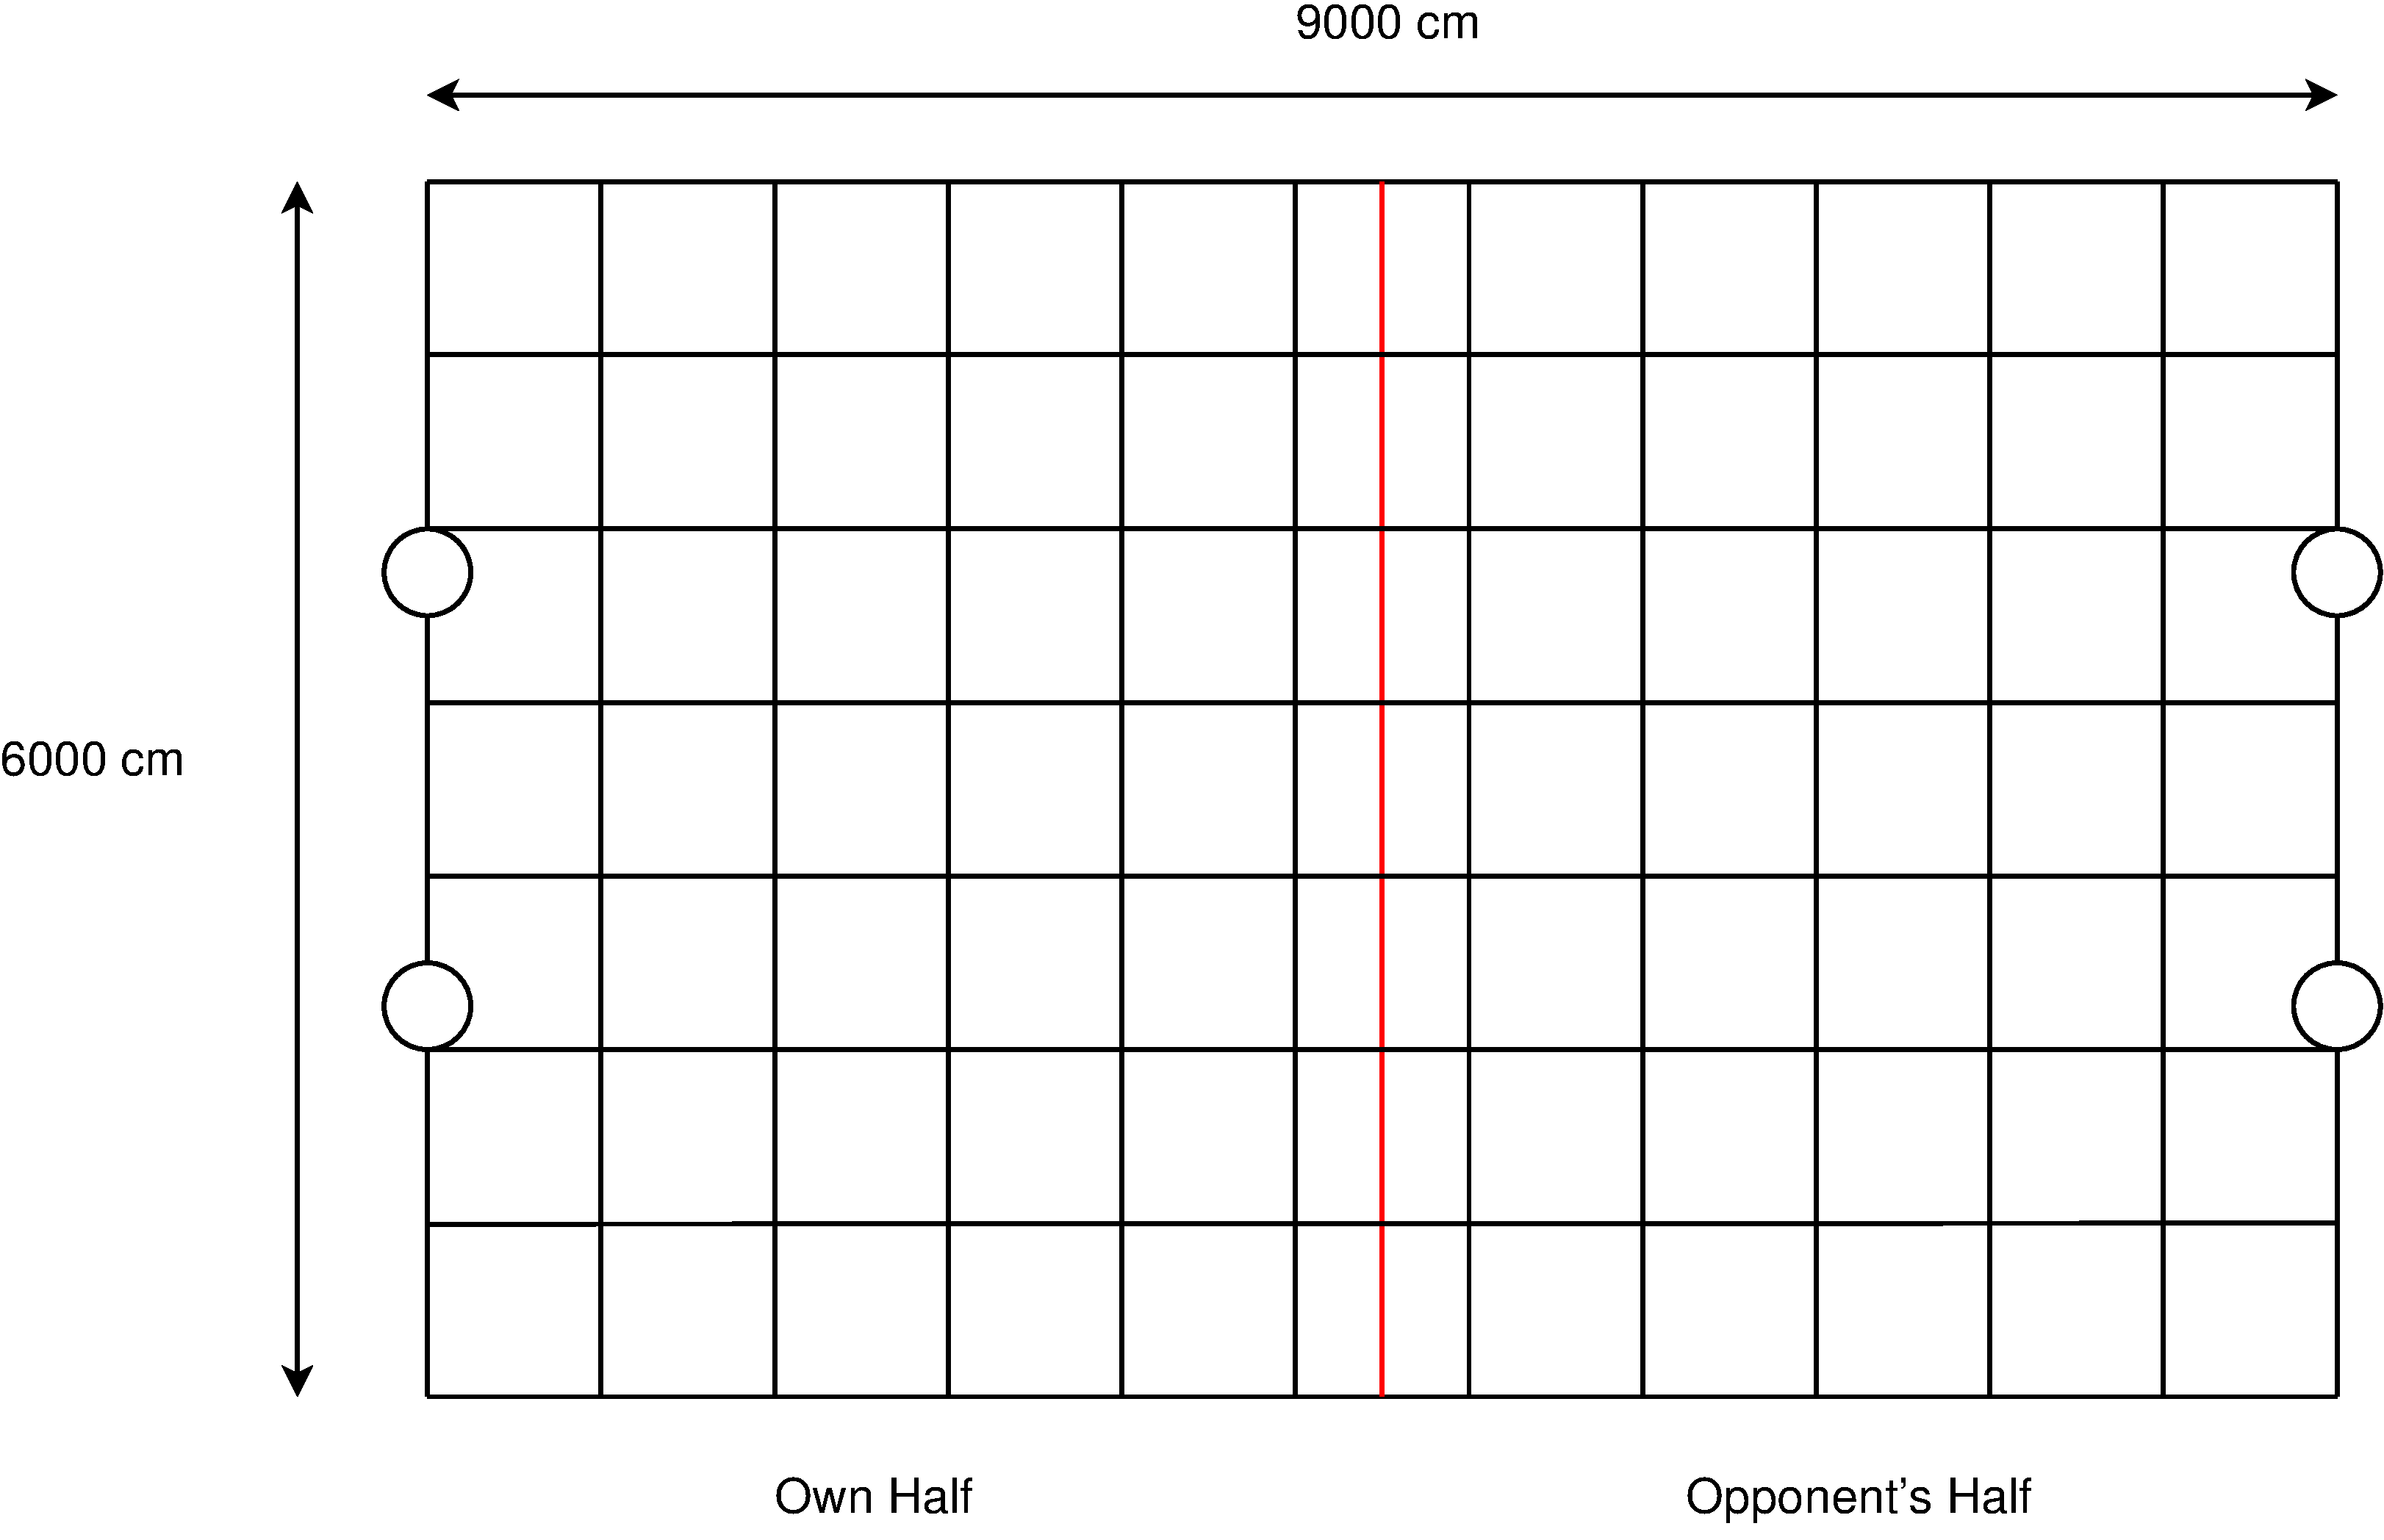
\includegraphics[width=0.7\textwidth]{gridworld.pdf}}
	{\caption{The grid world divides the field into a certain amount of cells.}\label{fig:gridworld}}
\end{figure}
We had different iterations of the grid world with different origins. At first the origin cell was in the lower left corner. Then we decided it would be better if the origin cell were in the middle of our own goal, mostly because it made calculations needed to determine the position of the robots easier. But if we wanted to use these calculations for both goals, it is easier to have the origin cell in the middle. 
\\
There is also a difference between choosing an even number and uneven number respectively on the x and the y direction. We decided to choose an uneven number for both, which means the origin cell is now in the middle of the centre spot. One benefit of that is that there is a cell that is exactly in the middle of the goal where the goalie stands most of the time. 
\\
Also when we take the cell at position (0,0) for example and we compare it to a similar coordinate system, then the upper right edge of that cell would be at (0.5, 0.5) in the coordinate system. When we calculate positions we don't get integers but decimal digits. 
So when we determine a robot's position on the field, we can simply round that result and know into what cell we have to put it.
\\
We explained earlier how to calculate the robot's position, but all the results were in millimetre. To convert these values into a cell one can use equations~\ref{equ:xcell} and~\ref{equ:ycell}.
\begin{equation}
	x\_cell = \frac{x\_mm}{field\_length} * x\_cell\_count
	\label{equ:xcell}
\end{equation}
\begin{equation}
	y\_cell = \frac{y\_mm}{field\_width} * y\_cell\_count
	\label{equ:ycell}
\end{equation}
\\
To store the data we use a dictionary in Python. The indexes of the dictionary are the positions in the grid world. For example (0,0) would be the centre of the field. Then we use numbers to fill that dictionary. At initialization the dictionary will be filled with zeroes, which is representing that there is nothing at that particular position. Here is a quick overview of the numbers we fill the dictionary with and what they mean:\\
0: nothing\\
1: own goal\\
2: enemy goal\\
3: own position\\
4: team mate\\
5: opponent\\
6: unclassified obstacle\\
7: ball\\
\\
So if we want to know the state of a certain position we call that dictionary and get back a number between 0 and 7. At the moment we don't use the numbers 6 and 7, but they could be useful in the future.
\\
Every robot can determine their own position themselves. The position of the team members is shared over the Wi-Fi, which will be explained in the next section. The robots can determine the position of opponents that they see. They share those positions so everyone has the position of as many opponents as possible. The robots actually can't distinguish between team mate and opponent. But because we know all the positions of our team members the robots can compare the position of the robots they see with the location of their team mates in their grid world. Only if there isn't a team mate in that cell they will identify the robot as an opponent. 
\\
This is one of the advantages of this representation of the field. The inaccuracy makes it easier to compare the found objects on the map between team mates. If we would measure everything in millimetre, every robot would probably calculate slightly different positions for the objects and so matching them would become more difficult.




%%%%%%%%%%%%%%%%%%%%%
%%%               %%%
%%% Communication %%%
%%%               %%%
%%%%%%%%%%%%%%%%%%%%%

\subsection{Communication}
\label{sec:solutions_communication}
Communication has always been one of the most important fields of research in RoboCup, at least it was the main reason to found the institution to find out whether two or more robots might possibly be able to act together in a senseful way. 
\\
Due to the increasing number of robots one team is allowed to have on the field (up two eleven in 2050, as the roadmap plans) and the high costs for one robot, it will become more and more necessary to cooperate with other teams. When there were the first tries of mixed teams some years ago, it was very fast obvious, that robots from different teams will have to communicate with each other.
\\
So some years ago, a RoboCup Soccer Humanoid Kid Size team implemented a Wi-Fi communication standard, the so called MiteCom,  that is used by a lot of teams in this league and makes it very easy to play in one team with robots from different teams. 
\\
So our idea was, that every robot could provide its own grid world and in return receive every other robots grid worlds. By weighting the incoming data due to reliability (like taking the median for each position of \textit{n} incoming grids) or currency ("I did not see a goal for a long time, i don' t know whether my own position is right or not, i will take a new grid and search for a goal") the average information quantity and quality could increase a lot.
\\
But our a big problem was, that via MiteCom it is only possible to send 32 bit integer values. Foremost we thought about implementing our own standard, but when thinking about it a second time, it seemed a good idea to use it. First of all, because of the aspect of universality mentioned above, that will be needed in the future. But furthermore it is not a bad idea to only send integers. 
\\
As already mentioned, on competitions the quality of WIFI is not very hight. So the big package loss could cause incompletely received data, and so only sending "small" 32 bit integers is more practicable. 
\\
The problem appeared, how to encode the dictionary, that represents the grid world, into an integer.
\\
Our solution is based on binary numbering system. Each of the 32 positions represents one cell in the Grid World. But dividing the hole $54m^2$ field in only 32 cells seemed very few. So we decided to use eight integers, each representing one eighth of the field.
\\
Besides, the binary integer can only depict one kind of information (numbers 1-7, see chapter Grid World) at a time. So we also need one integer per information type.
\\
When calculating these integers, the current part of the grid is scanned for the certain kind of information. When a grid-cell with the certain number is found, the grid cells number becomes the exponent of 2 and the sum of all of them gives the 32 bit integer, that is sent via MiteCom.
\\
When receiving data and updating the own Grid World, there is a hierarchy of persistence between opponent robots, team mates and the own position. 
\\
A new opponent robot is only written into the Grid World, when its position is not occupied with a team mate or the robots own position. After it is written into the Grid World, it is checked, whether it is a "new" opponent or it only has moved. To do so, the 8 surrounding cells are searched for opponent robots. We assume, that a robot would only move one cells per iteration. So if there was one in the surrounding cells before, it has moved to the new cell now and the old cell will be set to 0 (empty) again.
\\
However, when a team mate is added to the Grid World, the only value it cannot overwrite is the robots own position.

%%%%%%%%%%%%%%%
%%%         %%%
%%% Results %%%
%%%         %%%
%%%%%%%%%%%%%%%

\section{Results}

\subsection{Vision}
\label{sec:results_vision}
The vision of the bitbots software is completely renewed at the moment and as a result of that our current vision solutions would most likely be not compatible with the new vision. Unfortunately, as the new vision is still in an early testing stage, we were not able to implement the new vision in our project.
\\
Independently, the searching of the bottom of detected objects implemented by us remains an interesting feature that supplied better data, especially in combination with the filters it is robust and reliable enough to enable localisation.
\\
However the current vision software has issues and is not able to track objects like the goal posts stable/perfectly but perhaps some of the implemented concepts would also improve the development of the new vision. At least the interface of the current vision to the filters is dynamically build and thus adapting our filters to a similar interface to the new vision can be done easily.

\subsection{Filtering}
\label{sec:results_filtering}
Overall our customized DBSCAN algorithm with integrated arithmetical mean performed well when tested in a real world environment. The results (see figure~\ref{fig:dbscan_plot1}) improved our data and finally enabled us to develop a localisation. Furthermore its results for non-moving objects like the goal posts were far better than the results of a simple linear regression tried at first.
\\
On the contrary the cost of computation time of DBSCAN is far higher compared to simpler methods, for example smoothing the data with an arithmetical mean only.
\\
In addition to that the DBSCAN algorithm is at the moment nearly useless when it comes to moving objects or obstacles, like a ball because of the camera only recording about 20 frames per second the DBSCAN algorithm nether has enough data sets of the object to filter it appropriately. For filtering moving objects with DBSCAN a much higher framerate and thus a faster processor is needed to produce acceptable results.
\\
For our work respectively for the darwin-op the conclusion is to not overuse DBSCAN and to use other filters for moving objects, especially for fast moving objects. The speed of robots is slow enough to filter those data via DBSCAN but the quality of results is not worth the computation time it costs. Fast moving objects like balls should not be filtered with the DBSCAN.
\begin{figure}
 	\centerline{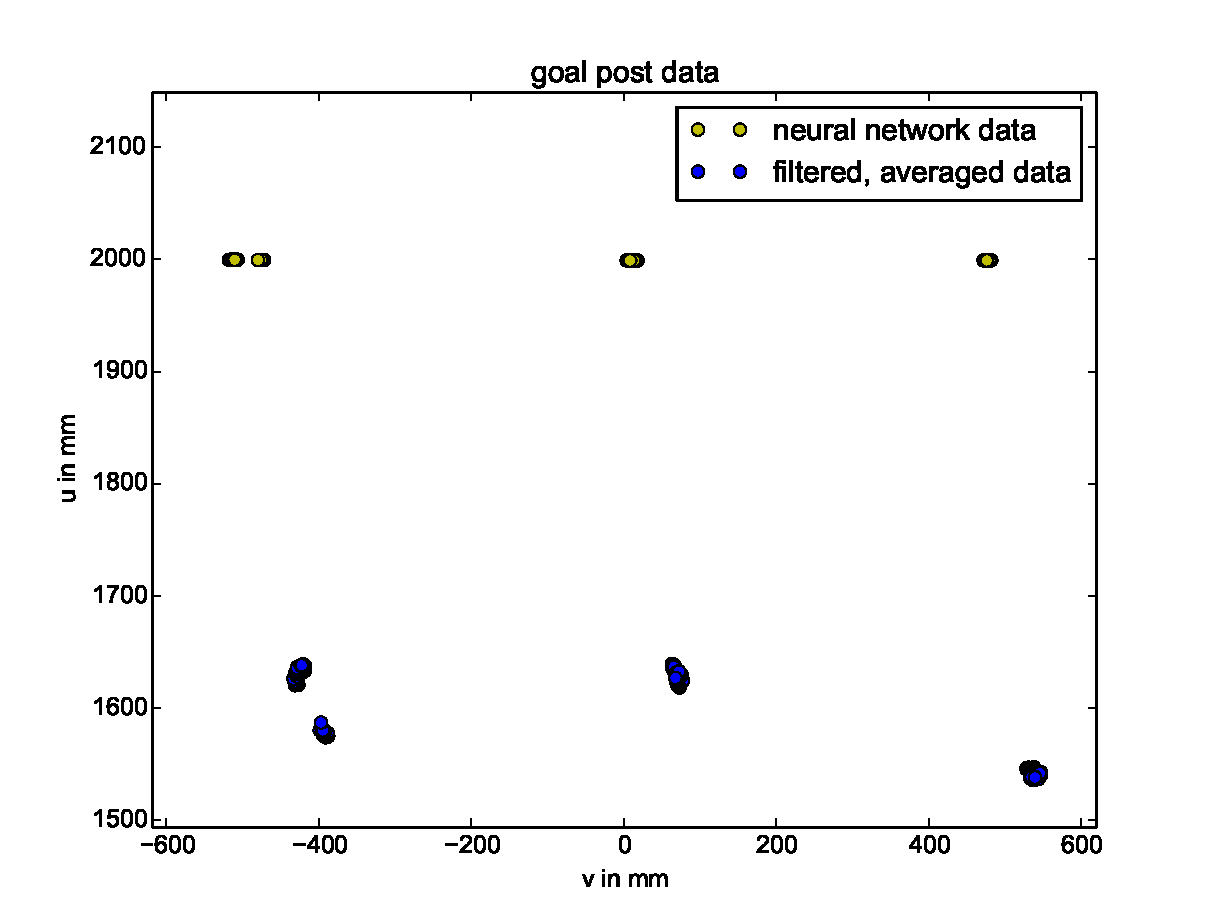
\includegraphics[width=0.7\textwidth]{ann_plot1.pdf}}
	{\caption{Plot of our neural network output with calibrated vision data compared to the just DBSCAN-filtered data. Goal posts have been placed at the positions (2000, -500), (2000, 0) and (2000, 500). The only DBSCAN filtered data (blue) has a higher standard deviation and misses the target values because of calibration issues. The DBSCAN and neural network filtered data has about half the standard deviation and is automatically calibrated by the neural network. }\label{fig:ann_plot1}}
\end{figure}
\\
To further boost the filtering results and to avoid manual (camera, ...) calibration a neural network can be used.
\\
As shown in figure~\ref{fig:ann_plot1} our neural network easily calibrates the vision if sufficient training data is recorded. This renders manual calibration obsolete and saves time. In addition to this the standard deviation of DBSCAN and averaged data is less than 5mm most of the time (and less 10mm in nearly all test scenarios) when objects are recorded in range of less or equal $2.5$m and the neural network improves this to a standard deviation of less than 3mm for those objects.
\\
Overall the neural network supplies an improvement of 25 to 50\% in accuracy (if measured via standard deviation) for DBSCAN-filtered objects in range of less or equal $2.5$m. Unfortunately we did not manage to do a full comparison of DBSCAN and DBSCAN plus neural network data as this would have exceeded the 20 pages limit and especially the deadline of our paper.
\\
Nevertheless in figure~\ref{fig:ann_plot1} at least the smaller sizes of the filtered clusters generated by the neural network can be perceived.
\begin{figure}
 	\centerline{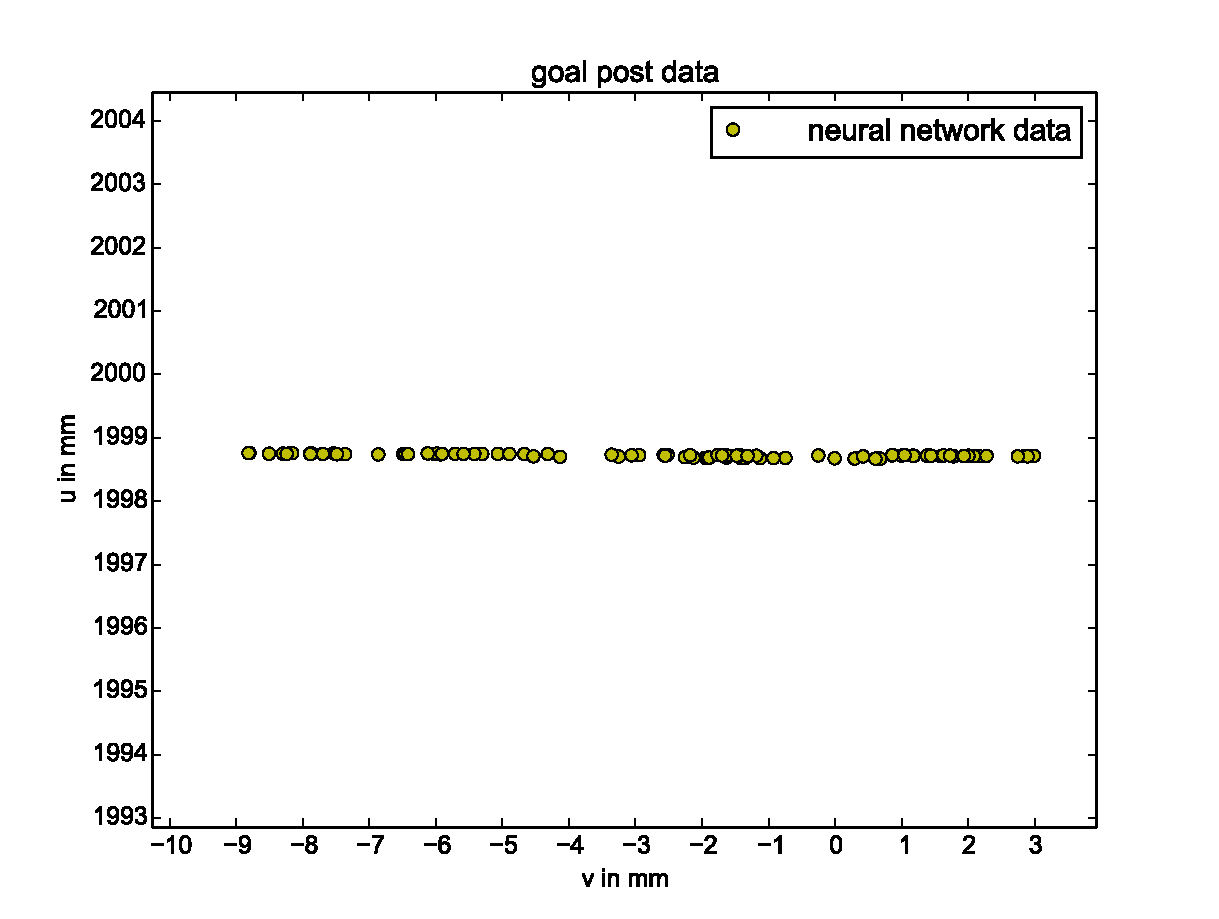
\includegraphics[width=0.7\textwidth]{ann_plot2.pdf}}
	{\caption{Plot of an overfitted neural network. Heavily magnification of a cluster of datasets, filtered by DBSCAN and the the neural network. Object (goal post) was recorded in a distance of (2000, 0).}\label{fig:ann_plot2}}
\end{figure}
\\
In opposition to the features, figure~\ref{fig:ann_plot2} demonstrates that neural networks can easily be overfitted. It is relatively hard to determine the best configuration for teaching the neural network. In our case of goal post / center localisation overfitting is not a big problem, because our gridworld already abstracts from real coordinates and maps it in the grids. So with a sufficient amount of training data the neural network could be overfitted to learn to map real coordinates directly to the grids of the gridworld rather than filtering it.
\\
However this scenario should not be implemented in release versions of the software until it is sufficiently tested. Overfitting of neural networks can drastically reduce the quality of produced data after training the network if the data passed to the network differs to much from training data.
\\
Supplementary the cost of computation time is higher compared to the easier filtering methods which were already mentioned and of course manual calibration would cost no computation time at all. Considering those negative side effects the neural network should not be overused as well.
\\
In contrary to the DBSCAN the neural network can also learn to filter and calibrate the positions of fast moving objects. Testing results with the ball were promising but not stable at different distances. The errors decrease with bigger neural nets but this would also heavily increase the computation time.
\\
Moreover the neural network needs a vast amount of training data to deliver accurately filtered and calibrated data. This can also be a time intensive task as collecting the training data takes quite some time.
\\
Conclusive the DBSCAN algorithm can be used for filtering goal information without issues. The neural network should only be used if sufficient training data was supplied. Additionally new training data has to be recorded over time because when the hardware changes the calibration error changes, too.
\\
Furthermore future improvements in the hardware could enable us to make new and bigger neural network designs due to the faster processors. For moving objects recurrent neural networks would improve the precision. According to the non-moving objects deep-learning networks could potentially improve the accuracy. Also reinforcement learning or at least some kind of auto-learning for the neural network would be increase the software's quality.
\\
The DBSCAN would most likely profit from a new camera and more frames per second.


\subsection{Localisation}
\label{sec:results_localisation}
Our localisation is able to compute the position of our own robots and furthermore the location of opponents. Unfortunately we didn't have enough time to implement this information into the behaviour. But there are several possibilities to use the data to our advantage. In the grid world module there is already a simple path finder implemented, that uses the A* search algorithm and avoids the occupied cells in the grid world. Another possible usage could be to coordinate which player should go to the ball depending on who has the shortest path. And there's a lot more potential to benefit from the grid world.
\\
We also implemented a solution that computes the position of our robot with vectors instead of angles. But this was towards the end of our project so we didn't have enough time to explain it in this paper.
\\
Unfortunately we didn't have enough time to conduct our tests of the grid world to the end. So there are still some bugs. 
\\
Also the tests were only successful when the robot had good sight of the goal. In the code there is actually a line detection but we found out to late about it and there was no time left to improve our localisation with it. Another aspect that needs to be implemented is to figure out a way for the robot to know which goal it is looking at.
\\
So there is still a lot of room for improvements, but this was something we expected at the start of the project. It's unfortunate that there wasn't more time to test our localisation and fix the rest of the bugs, but apart from this we are satisfied with the resulting localisation.


\subsection{Communication}
\label{sec:results_communication}
For the communication part it can be said, that the basis for a lot of further work is done. At the moment sharing information on localisation increases the quality and quantity of every single robot and thus of the whole team. The error rate is being reduced and so the information becomes more reliable. It is hard to quantify the advantage, but the next competition will hopefully give the answer. At least it will be very hard for the robots trying to score on their own goal.
\\
Something that needs to developed in further work is the question of data integration. Our solution with the very simple overwriting hierarchy between opponents, team mates and the robots own position is good enough for the beginning of development is this area, but soon will come to its limitations, especially when there are several robots standing close to each other. In this situation our assumption of a robot moving one cell per iteration would be wrong, because it was not a movement of one robot, but really two robots standing close to each other. So opponent robots could be deleted. 
\\
One idea to avoid this to happen might be, to have a minimum and maximum amount of team mates and opponents and a rating for each of them. When there are too many, only the best ones are taken and only the worst one can be deleted.
\\
In general it should be thought about an algorithms that take the last \textit{n} received grid worlds and weights them before the own grid world is updated.  Depending on the quality of Wi-Fi (the last \textit{n} grid worlds, but not older then \textit{m} seconds), the information could be averaged or even more filtered (like taking the median). 
\\
Or the robots could use an internal rating system for the incoming data. One heuristic might depend on prioritising the goalie, as it often stands still, has a good view over the field and does not move too much. This makes his information more reliable then the other robots information. 
\\
But all of these ideas could not have been part of this project due to the limited time. In the future the our results seems to bring a big effort for the team and surely will be extended further.
our results
behaviour


%%%%%%%%%%%%%%%
%%%         %%%
%%% Summary %%%
%%%         %%%
%%%%%%%%%%%%%%%

\section{Summary}
Although many of the modules can be improved and some failures still remain our software provides useful data. The vision produces more reliable data because of our implementation which searches for the bottom of an object. The DBSCAN algorithm and the afterwards calculated arithmetical mean supplies enhanced, filtered data in comparison to the raw data which makes positioning possible. The neural network additionally increased the accuracy of our filtered data and solved the calibration issues.
\\
The grid world module consumes this filtered data and processes the information to determine the robots position on the field. Once the robots position is found this enables us to deduce other object's positions (obstacles, enemies, team mates, ball, ...). This is the key for intelligent behaviour.
\\
The communication module provides each robot's information for the whole team and thus helps visionless robots to relocate. In addition it increases the average quality of information and makes team coordination possible.




%%%%%%%%%%%%%%%%%%%%
%%%              %%%
%%% Bibliography %%%
%%%              %%%
%%%%%%%%%%%%%%%%%%%%

\begin{thebibliography}{5}

\bibitem{ester:kriegel} Ester, M., Kriegel, H.-P., Sander, J., Xu, X.:
A Density-Based Algorithm for Discovering Clusters in Large Spatial Databases with Noise.
In: Proceedings of 2nd International Conference on Knowledge Discovery and Data Mining (KDD-96),
pp. 226--231. AAAI Press, Munich (1996)

\bibitem{mlp} Grosan, C., Abraham, A.:
Intelligent Systems - A Modern Approach.
pp. 299--316. Springer Berlin Heidelberg, Volume 17 (2011)

\bibitem{grid} Salehi, M.E., Safdari, R., Abedi, E., Foroughi, B., Salimi, A., Farokhi, E., Teimouri, M., Shakiba, R.: MRL Team Description Paper for Humanoid KidSize League of RoboCup 2014. 
Mechatronics Research Lab, Dept. of Computer and Electrical Engineering,
Qazvin Islamic Azad University, Qazvin, Iran (2014)

\bibitem{tree} van der Molen, H.: Self-localization in the RoboCup Soccer Standerd Platform League with the use of a Dynamic Tree. A Bachelor Thesis in Artificial Intelligence, University Of Amsterdam (2011)


\end{thebibliography}





\end{document}
